\documentclass{article}

\usepackage{graphicx}
\usepackage{tikz}
\usepackage{tikzsymbols}
\usetikzlibrary{calc,patterns,shapes.geometric}
\pagestyle{empty}
\usepackage[margin=0pt]{geometry}
\geometry{papersize={14in,12in}}

\def\centerarc[#1](#2)(#3:#4:#5){\draw[#1] ($(#2)+({#5*cos(#3)},{#5*sin(#3)})$) arc (#3:#4:#5);}

\begin{document}
	\begin{figure}
		\centering
		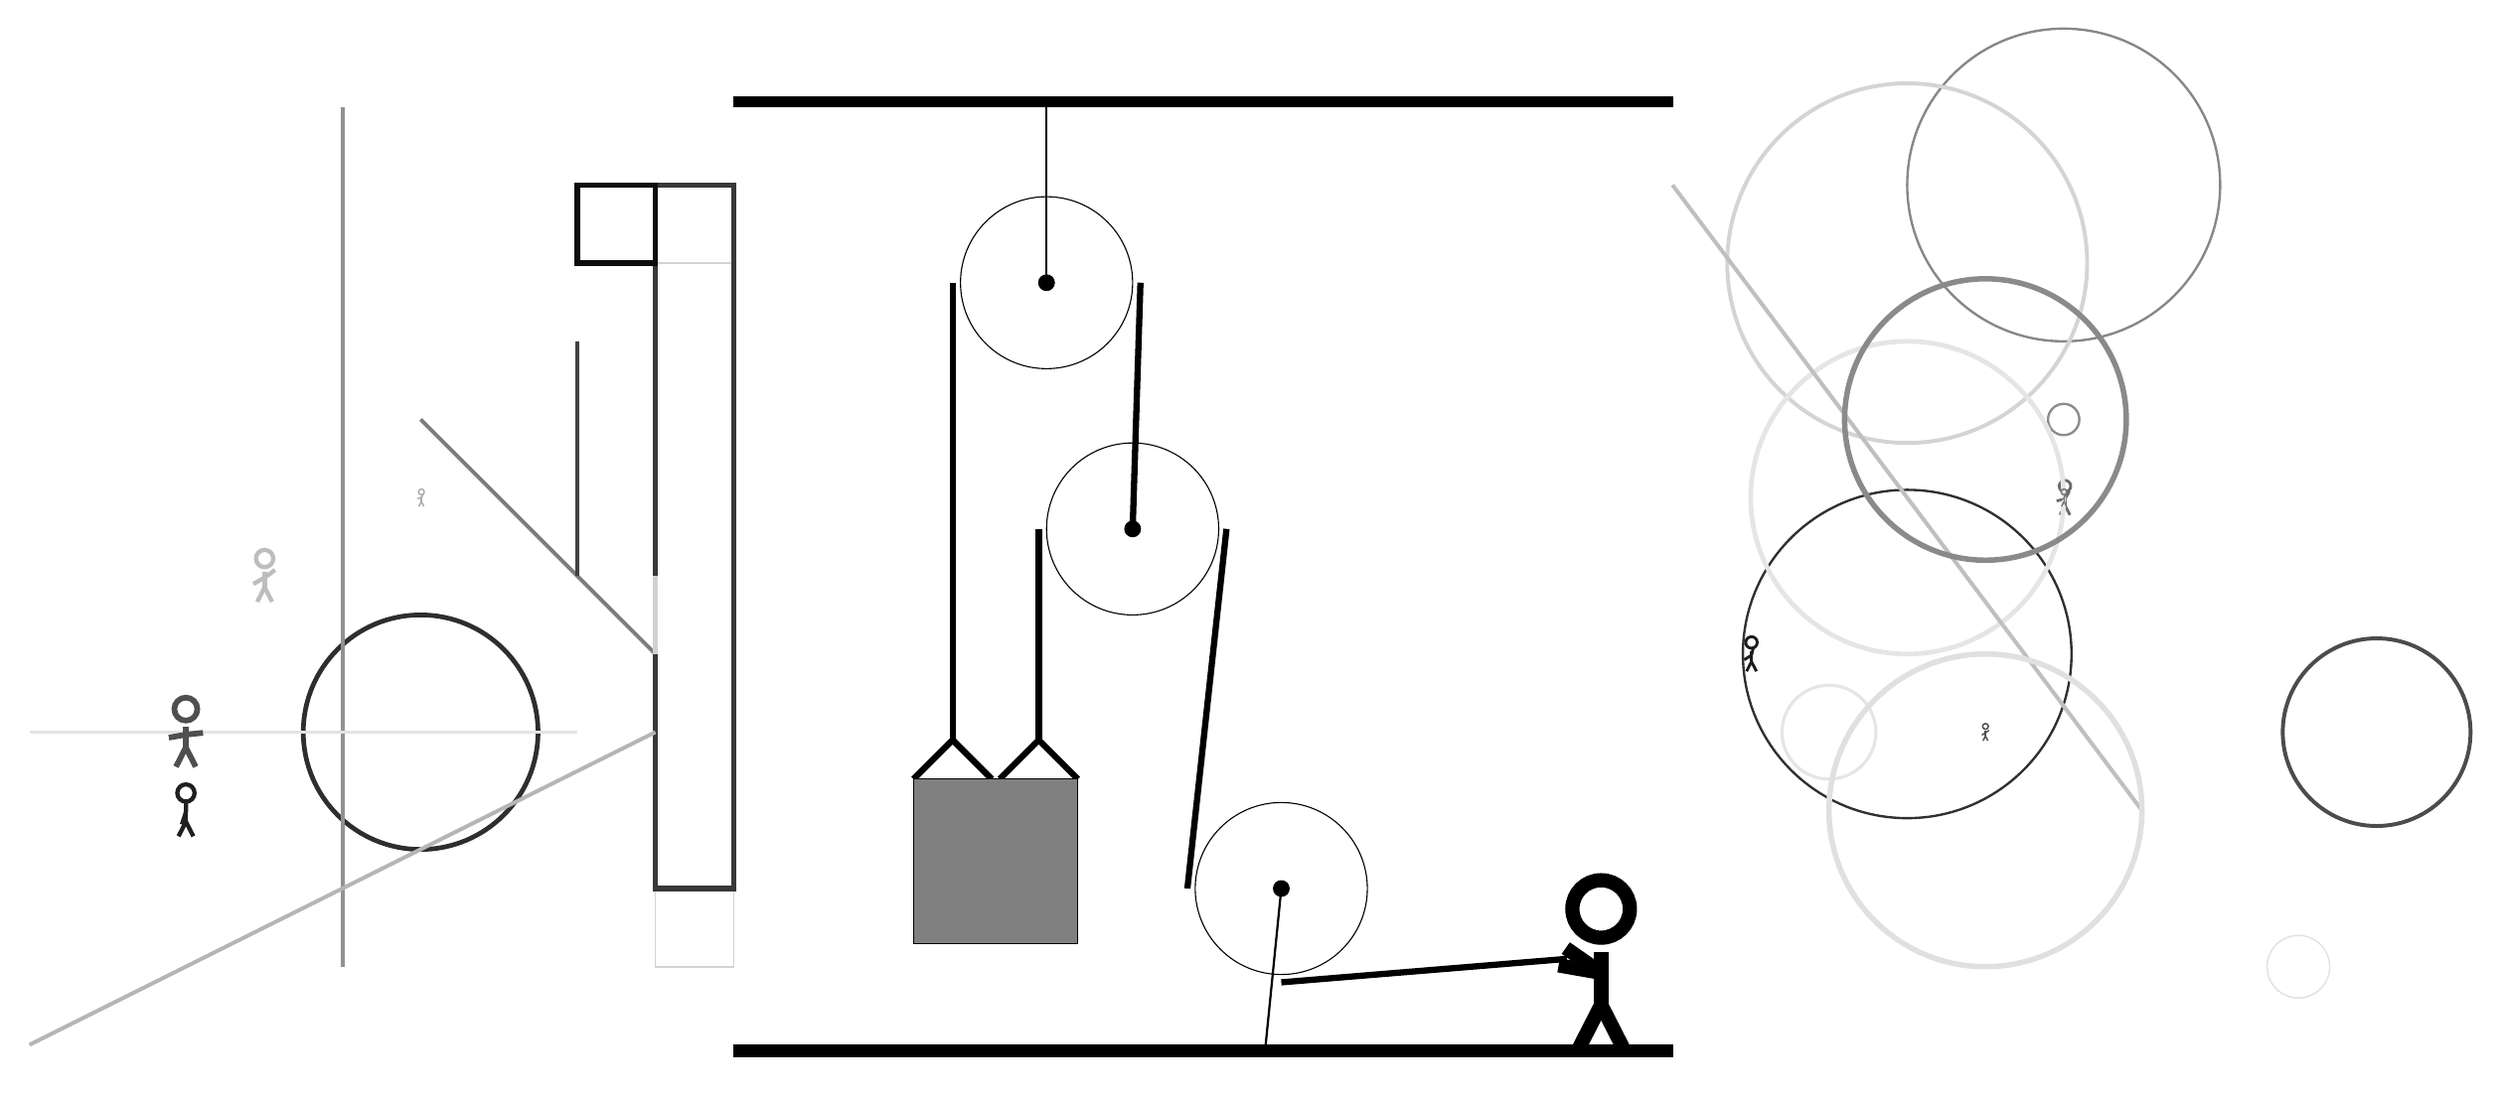
\begin{tikzpicture}
			%%%%% START %%%%%
			
			\draw[fill=black] (-2, 9) rectangle (10, 9.125);
			
			\draw (2, 6.75) circle (1.1);
			\draw[fill=black] (2, 6.75) circle (0.1);
			\draw[thick] (2, 6.75) -- (2, 9);
			
			\draw [line width=0.3mm, color=black!47](15, 8) circle (2.0);
			
			\draw [line width=0.6mm, color=black!82](-6, 1) circle (1.5);
			\draw [line width=0.3mm, color=black!45](15, 5) circle (0.2);
			\node[line width=0.4mm, color=black!88] at (-9, 0) {\Strichmaxerl[3][72][89]};
			\draw[line width=0.5mm, color=black!51](-6, 5) -- (-3, 2);
			
			\draw [line width=0.4mm, color=black!10](12, 1) circle (0.6);
			\draw [line width=0.3mm, color=black!81](13, 2) circle (2.1);
			
			\draw[line width=0.5mm, color=black!43](-7, -2) -- (-7, 9);
			\node[line width=0.2mm, color=black!89] at (11, 2) {\Strichmaxerl[2][32][76]};
			\draw[line width=0.2mm, color=black!17] (-3, 7) rectangle (-2, -2);
			\node[line width=0.7mm, color=black!58] at (15, 4) {\Strichmaxerl[2][14][60]};
			
			\draw [line width=0.5mm, color=black!70](19, 1) circle (1.2);
			\draw [line width=0.5mm, color=black!17](13, 7) circle (2.3);
			
			\draw[line width=0.5mm, color=black!11](-4, 1) -- (-11, 1);
			\draw [line width=0.2mm, color=black!11](18, -2) circle (0.4);
			\draw [line width=0.6mm, color=black!10](13, 4) circle (2.0);
			
			\node[line width=0.7mm, color=black!33] at (-6, 4) {\Strichmaxerl[1][1][67]};
			\node[line width=0.7mm, color=black!55] at (15, 4) {\Strichmaxerl[1][32][73]};
			\draw[line width=0.5mm, color=black!74] (-4, 3) rectangle (-4, 6);
			\node[line width=0.2mm, color=black!70] at (14, 1) {\Strichmaxerl[1][33][35]};
			\draw[line width=0.7mm, color=black!78] (-2, 8) rectangle (-3, -1);
			
			\draw[line width=0.7mm, color=black!95] (-4, 7) rectangle (-3, 8);
			\node[line width=0.3mm, color=black!26] at (-8, 3) {\Strichmaxerl[3][29][37]};
			\draw[line width=0.5mm, color=black!25](10, 8) -- (16, 0);
			\draw[line width=0.5mm, color=black!29](-3, 1) -- (-11, -3);
			\draw [line width=0.7mm, color=black!12](14, 0) circle (2.0);
			
			\draw[line width=0.6mm, color=black!18] (-3, 3) rectangle (-3, 2);
			\node[line width=0.3mm, color=black!69] at (-9, 1) {\Strichmaxerl[4][10][6]};
			\draw [line width=0.7mm, color=black!46](14, 5) circle (1.8);
			
			\draw (3.1, 3.6) circle (1.1);
			\draw[fill=black] (3.1, 3.6) circle (0.1);
			
			\draw (5, -1) circle (1.1);
			\draw[fill=black] (5, -1) circle (0.1);
			\draw[thick] (5, -1) -- (4.8, -3);
			
			\draw[line width = 0.8mm]  (0.3, 0.4) -- (0.8, 0.9) -- (1.3, 0.4);
			\draw[line width = 0.8mm]  (1.4, 0.4) -- (1.9, 0.9) -- (2.4, 0.4);
			\draw[fill=black!50] (0.3, 0.4) rectangle (2.4, -1.7);
			
			\draw[line width = 0.8mm] (0.8, 6.75) -- (0.8, 0.9);
			\centerarc[line width = 0.8mm](2, 6.75)(0:180:1.2000000000000002);
			\draw[line width = 0.8mm] (3.2, 6.75) -- (3.1, 3.6);
			\draw[line width = 0.8mm] (1.9, 3.6) -- (1.9, 0.9);
			\centerarc[line width = 0.8mm](3.1, 3.6)(0:180:1.2000000000000002);
			\draw[line width = 0.8mm] (4.3, 3.6) -- (3.8, -1);
			\centerarc[line width = 0.8mm](5, -1)(180:270:1.2000000000000002);
			\draw[line width = 0.8mm] (5, -2.2) -- (8.65, -1.9);
			
			\node at (9, -2) {\Strichmaxerl[10][-35][170]};
			
			\draw[fill=black] (-2, -3) rectangle (10, -3.15);
			
			%%%%% END %%%%%
		\end{tikzpicture}
	\end{figure}	
\end{document}